\documentclass{article}
\usepackage{graphicx}

% Prawidłowe dzielenie polskich wyrazów na sylaby przy przenoszeniu do następnej linii
\usepackage[polish]{babel} 

% Aby akceptował polskie litery
\usepackage[utf8]{inputenc}
\usepackage[T1]{fontenc}

% Minimalizacja marginesów
\usepackage[portrait]{geometry}
\geometry{
    left=20mm,
    right=20mm,
    top=20mm,
    bottom=20mm,
    headheight=15pt,
    voffset=10pt,
    footskip=15pt
}

\begin{document}


\section*{0. Projekt 'Rezerwacja kortów tenisowych'}
Cel - Realizacja zadania z baz danych  laboratorium 

\subsection*{1. Opis zawartości}

Baza zawiera dane na temat wynajmów kortów tenisowych pozwalających na wykonanie analiz przychodów dotyczących wynajmu kortów nie zrealizowanych gier na kortach, posiada również informacje o klientach oraz wsparciu kortów pozwalając dokonywać analiz dotyczących ich wynajmu.


\subsection*{2. Ogólny opis domenty}

Wynajem kortów tenisowych buduje problem  związanych z efektywnym i planowym udostępnianiem powierzchni dla zainteresowanych graczy , tworzeniem statystyk wynajmu oraz badaniem jakości obsługi poprzez obserwacje incydentów związanych z utrzymaniem obiektu.
W ramach domeny nie uwzględniamy elementów kosztowych  które leżą w kompetencji działu finansowo księgowego które jako oprogramowanie specjalistyczne  wychodzi poza zakres naszej prostej aplikacji.


\subsection*{3. Możliwe zapytania w języku naturalnym}

\noindent

•	Pokaż raport analizy przychodów dotyczących wynajmu kortów tenisowych dla niezrealizowanych gier na kortach w określonym okresie czasu.\\
•	Udostępnij statystyki wynajmu kortów tenisowych, uwzględniając popularność różnych rodzajów kortów (np. nawierzchnia) oraz godziny największego obłożenia.\\
•	Pokaż raport dotyczący incydentów związanych z utrzymaniem obiektu kortów tenisowych, wraz z danymi na temat rozwiązanych i nierozwiązanych problemów.\\
•	Udostępnij zestawienie danych klientów, którzy korzystali z obsługi kortów tenisowych, wraz z opisem zgłoszonych problemów i ich statusami.\\
•	Pokaż historię rezerwacji danego klienta, wraz z informacjami o zrealizowanych i niezrealizowanych rezerwacjach.\\
•	Udostępnij raporty dotyczące obłożenia kortów w poszczególnych godzinach i dniach tygodnia, aby zoptymalizować planowanie dostępności kortów.\\
•	Pokaż rezerwacje zaplanowane na najbliższy tydzień, wraz z ich statusem.


\subsection*{4. Podstawowe kategorie obiektów i ich atrybuty}

\subsubsection*{Tabela: Korty}
•	KortID (Klucz główny, automatycznie generowany identyfikator)\\
•	NumerKortu (numer identyfikacyjny kortu)\\
•	TypKortu (np. nawierzchnia, oświetlenie)\\
•	CenaGodzinowa (cena za godzinę wynajmu)\\
•	Inne informacje związane z kortem\\

\subsubsection*{Tabela: Klienci}
•	KlientID (Klucz główny, automatycznie generowany identyfikator)\\
•	Imię\\
•	Nazwisko\\
•	Adres\\
•	Telefon\\
•	Email\\
•	Inne informacje o kliencie

\subsubsection*{Tabela: Rezerwacje}
•	RezerwacjaID (Klucz główny, automatycznie generowany identyfikator)\\
•	KortID (Klucz obcy, odniesienie do Kortu)\\
•	KlientID (Klucz obcy, odniesienie do Klienta)\\
•	DataRozpoczęcia (data i godzina rozpoczęcia rezerwacji)\\
•	DataZakończenia (data i godzina zakończenia rezerwacji)\\
•	Opłata (opłata za rezerwację)\\
•	StatusRezerwacji (status rezerwacji, np. Anulowana, Zrealizowana)\\
•	Inne informacje związane z rezerwacją\\

\subsubsection*{Tabela: Pracownicy}
•	PracownikID (Klucz główny, automatycznie generowany identyfikator)\\
•	Imię\\
•	Nazwisko\\
•	Stanowisko\\
•	DataZatrudnienia\\
•	Wynagrodzenie\\
•	Inne informacje o pracowniku

\subsubsection*{Tabela: ObsługaKortow}
•	MaintenanceID (Klucz główny, automatycznie generowany identyfikator)\\
•	KortID (Klucz obcy, odniesienie do Kortu)\\
•	PracownikId (pracownik, odpowiedzialny za realizację zadania)\\
•	DataRaportu (data zgłoszenia konieczności obsługi)\\
•	OpisProblemu (opis problemu, który wymaga obsługi)\\
•	Status (status obsługi, np. w trakcie, zakończona)\\
•	Koszty (koszty związane z obsługą)\\
•	Inne informacje związane z obsługą kortów

\section*{Zestaw zadań nr 2}

\subsection*{Formalne definicje}

Tabela: Korty\\
- KortId (klucz główny, automatycznie generowany identyfikator, np. 1)\\
- NumerKortu (numer identyfikacyjny kortu np Kort1, Kort2)\\
- TypKortu (Możliwości: Otwarty, Zamknięty)\\
- CenaGodzinowa (cena za godzinę wynajmu)\\

Tabela: Klienci\\
- KlientID (Klucz główny, automatycznie generowany identyfikator, np. 1)\\
- Imię (max 50 znaków)\\
- Nazwisko (max 50 znaków)\\
- Adres (max 200 znaków, opcjonalne)\\
- Telefon (max 20 znaków, opcjonalne)\\
- Email (max 50 znaków, opcjonalne)\\

Tabela: Rezerwacje (wszystkie pola wymagane)\\
- RezerwacjaID (Klucz główny, automatycznie generowany identyfikator, np. 1)\\
- KortID (Klucz obcy, odniesienie do Kortu)\\
- KlientID (Klucz obcy, odniesienie do Klienta)\\
- DataRozpoczęcia (data i godzina rozpoczęcia rezerwacji)\\
- DataZakończenia (data i godzina zakończenia rezerwacji)\\
- Opłata (opłata za rezerwację, np 50 PLN)\\
- StatusRezerwacji (Możliwości: Aktywna, Anulowana, Zrealizowana)\\

Tabela: Pracownicy\\
- PracownikID (Klucz główny, automatycznie generowany identyfikator)\\
- Imię (max 50 znaków)\\
- Nazwisko (max 50 znaków)\\
- Stanowisko (max 50 znaków, opcjonalne)\\

Tabela: ObsługaKortow\\
- MaintenanceID (Klucz główny, automatycznie generowany identyfikator)\\
- KortID (Klucz obcy, odniesienie do Kortu)\\
- PracownikId (pracownik, odpowiedzialny za realizację zadania)\\
- DataRaportu (data zgłoszenia konieczności obsługi)\\
- OpisProblemu (opis problemu, który wymaga obsługi)\\
- Status (Możliwe: Zgłoszone, Aktualne, Rozwiazane)\\
- Koszty (koszty związane z obsługą zgłoszenia)\\

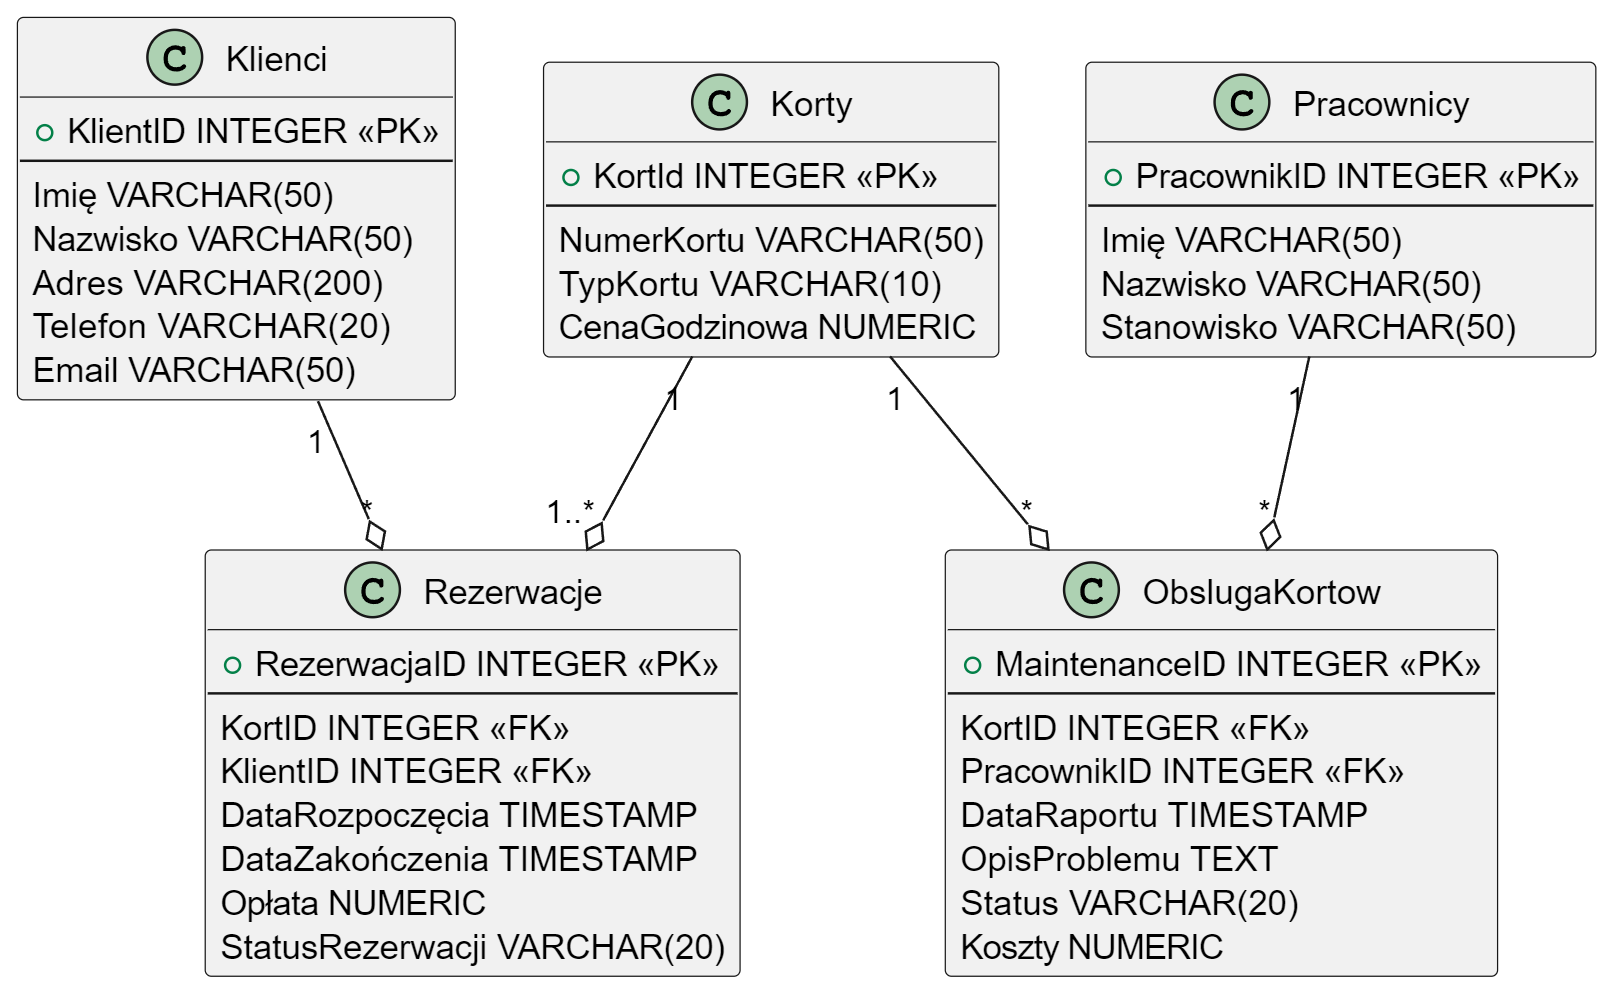
\includegraphics{diagram.png}

\end{document}